\begin{figure}[tbp]
\centering
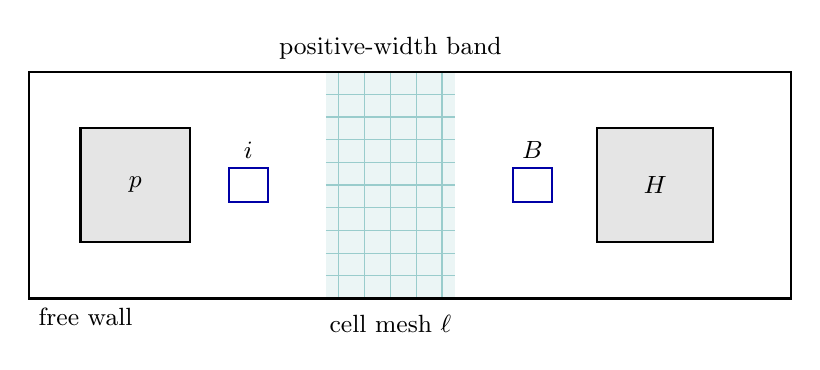
\begin{tikzpicture}[x=.82cm,y=.72cm,font=\small]
 \fill[teal!8] (4.6,0) rectangle (6.6,4);
 \draw[teal!40,step=.4] (4.6,0) grid (6.6,4);
 \draw[thick] (0,0) rectangle (11.8,4);
 \filldraw[fill=black!10,draw=black,thick] (.8,1) rectangle (2.5,3);
 \filldraw[fill=black!10,draw=black,thick] (8.8,1) rectangle (10.6,3);
 \draw[blue!65!black,thick] (3.1,1.7) rectangle (3.7,2.3);
 \draw[blue!65!black,thick] (7.5,1.7) rectangle (8.1,2.3);
 \node at (1.65,2) {$p$};
 \node at (9.7,2) {$H$};
 \node[above] at (5.6,4.05) {positive-width band};
 \node[above] at (3.4,2.3) {$i$};
 \node[above] at (7.8,2.3) {$B$};
 \node[below] at (5.6,-.12) {cell mesh $\ell$};
 \node[below right] at (0,0) {free wall};
\end{tikzpicture}
\caption{The band separates two positive-area pin regions.
The test boxes lie away from the band. Its cell mesh \(\ell\)
is refined while the physical band width stays fixed; the
band strength is increased only afterwards. Hard pins constrain
all primary height vertices in their regions.}
\label{fig:band}
\end{figure}
